% Name: Transpose of a matrix
% Description: The transpose turns rows into columns: the first row of the 2×3 matrix A is the first column of the 3×2 matrix Aᵀ, and the entry in row i, column j moves to row j, column i.
% Tags: transpose, rows and columns, matrix, linear algebra

\usetikzlibrary{matrix, fit, backgrounds, positioning, arrows.meta}

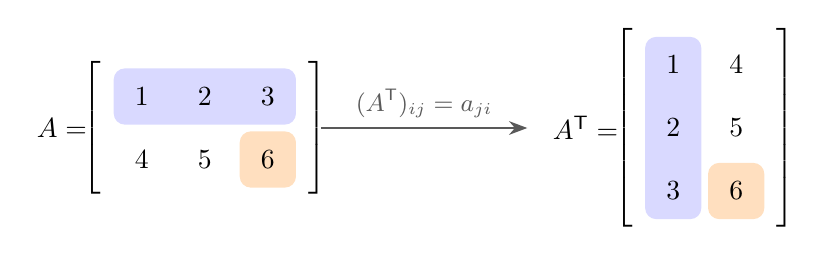
\begin{tikzpicture}[>={Stealth}, mat/.style={matrix of math nodes, left delimiter={[}, right delimiter={]}, nodes={minimum size=7mm}, column sep=1mm, row sep=1mm}]
  \matrix[mat] (A) {
    1 & 2 & 3 \\
    4 & 5 & 6 \\
  };
  \node[left=1mm of A] {$A =$};
  \matrix[mat, right=4.2cm of A] (T) {
    1 & 4 \\
    2 & 5 \\
    3 & 6 \\
  };
  \node[left=1mm of T] (eq) {$A^{\mathsf{T}} =$};
  \begin{scope}[on background layer, every node/.style={rounded corners, inner sep=0pt}]
    \node[fill=blue!15, fit=(A-1-1)(A-1-3)] {};
    \node[fill=blue!15, fit=(T-1-1)(T-3-1)] {};
    \node[fill=orange!25, fit=(A-2-3)] {};
    \node[fill=orange!25, fit=(T-3-2)] {};
  \end{scope}
  \draw[->, thick, gray!70!black] ([xshift=2mm]A.east) -- node[above, font=\small] {$(A^{\mathsf{T}})_{ij} = a_{ji}$} ([xshift=-2mm]eq.west);
\end{tikzpicture}
